\subsubsection{Um Guia de Boas Práticas de Código para OutSystems}\label{secsec:um-guia-de-estilo-de-codigo}

    Todas as linguagens de programação bem estabelecidas têm diretrizes de programação tão bem enraizadas na cultura da língua que são ensinadas em conjunto com ela, desta forma, com os profissionais a aplicar um método parecido no desenvolvimento do código tem-se um projeto muito mais coerente.

    No entanto, OutSystems carece de um guia de diretrizes estabelecido. Isto deve-se principalmente ao facto de OutSystems ser radicalmente diferente de outras linguagens de programação, sendo um paradigma visual onde até a interface pode ser modificada, não existe um consenso universal para a forma como o código deva ser organizado visualmente.

    Neste capítulo vamos explorar algumas das diretrizes que nos foram introduzidas e aconselhadas a seguir quando alterássemos código na aplicação. Estas indicações começaram a ser introduzidas recentemente, pelo que muito do código existente não cumpre estas normas, mas há um incentivo para uniformizar o código da aplicação.

    \textbf{Diretriz 1 — Sentido descendente é progresso:} Figura \ref{fig:diretriz1}, o sentido descendente deve levar-nos ao objetivo da ação. Este é o sentido de leitura geralmente acordada, até por diferentes culturas;

    \textbf{Diretriz 2 — Ramificações para a direita:} Figura \ref{fig:diretriz2}, o ramo mais importante de um ``if'' deverá seguir da esquerda para a direita. Um nodo ``if'' geralmente tem um ramo que se espera ser executado com mais frequência ou o ramo que é simplesmente mais importante a termos de valor comercial. Este ramo deve mover-se para a direita, e o outro deve 
    continuar reto para baixo;

    \begin{figure}[H]
        \centering
        \begin{minipage}{.5\textwidth}
            \centering
            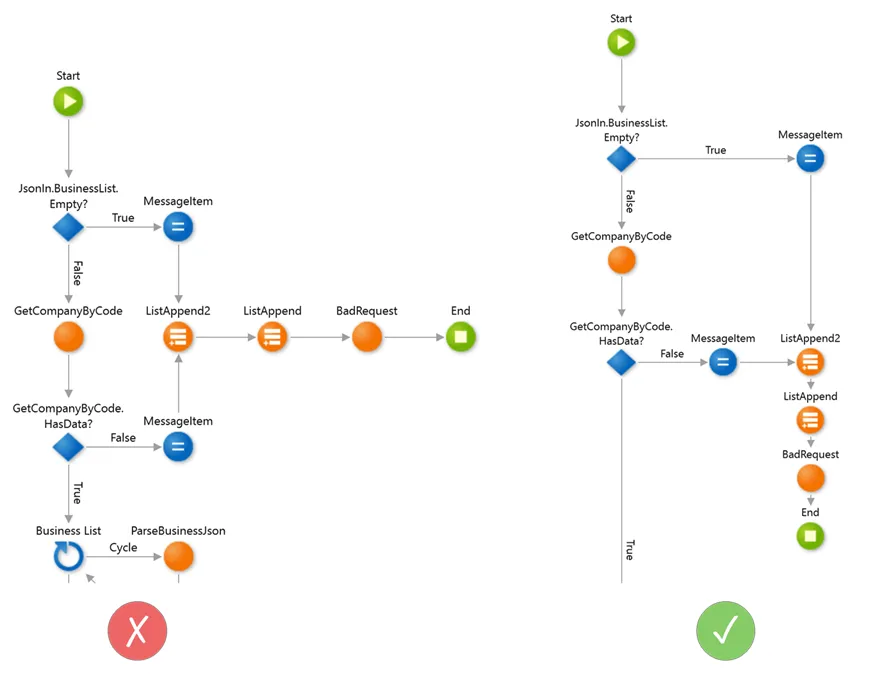
\includegraphics[scale=0.35]{imgs/diretrizes/1.png}
            \caption{Diretriz 1 — Sentido descendente é progresso}\label{fig:diretriz1}
            \source{\cite{outsystems-style-guide}}
        \end{minipage}%
        \begin{minipage}{.5\textwidth}
            \centering
            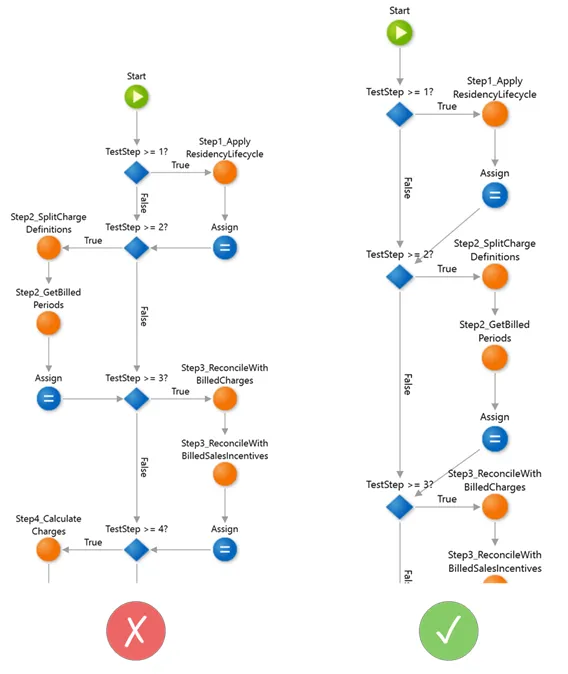
\includegraphics[scale=0.40]{imgs/diretrizes/2.png}
            \caption{Diretriz 2 — Ramificações para a direita}\label{fig:diretriz2}
            \source{\cite{outsystems-style-guide}}
        \end{minipage}
    \end{figure}

    \textbf{Diretriz 3 — Exceções para a direita:} Figura \ref{fig:diretriz3}, exceções para a direita, mesmo que não seja o ramo ``mais importante''. Se se aplicasse a diretriz 2 às exceções, acabava-se com um código maioritariamente horizontal, desta forma impede-se destacar a exceção, e mantém-se o foco no código principal;

    \textbf{Diretriz 4 — Ciclos:} Figura \ref{fig:diretriz4}, ciclos devem iniciar-se numa diagonal para cima e para a direita;

    \begin{figure}[htbp]
        \centering
        \begin{minipage}{.5\textwidth}
            \centering
            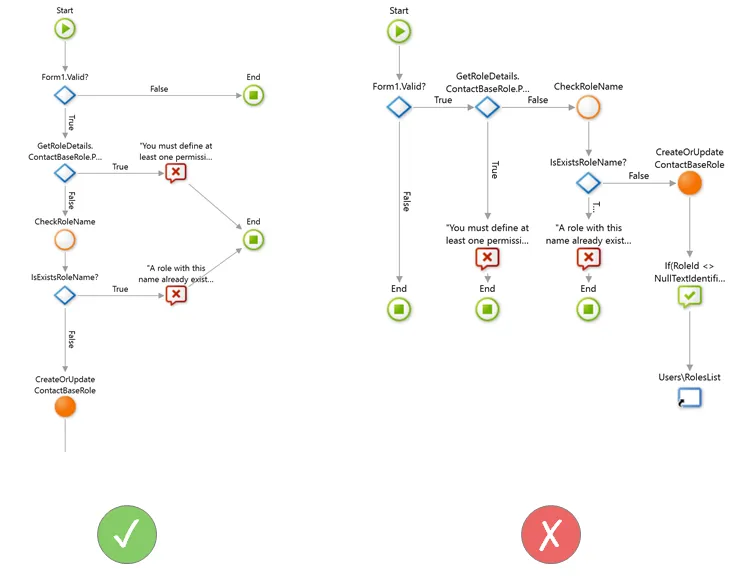
\includegraphics[scale=0.40]{imgs/diretrizes/3.png}
            \caption{Diretriz 3 — Exceções para a direita}\label{fig:diretriz3}
            \source{\cite{outsystems-style-guide}}
        \end{minipage}%
        \begin{minipage}{.5\textwidth}
            \centering
            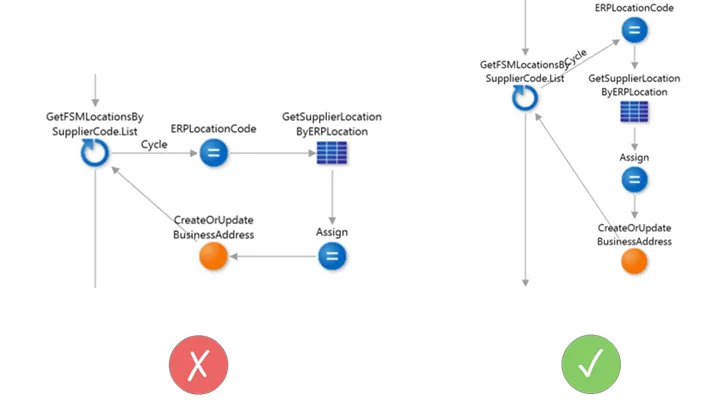
\includegraphics[scale=0.32]{imgs/diretrizes/4.png}
            \caption{Diretriz 4 — Ciclos}\label{fig:diretriz4}
            \source{\cite{outsystems-style-guide}}
        \end{minipage}
    \end{figure}

    \textbf{Diretriz 5 — Evitar setas sobrepostas:} Figura \ref{fig:diretriz5}, setas sobrepostas devem ser evitadas mesmo que implique ignorar outra diretriz, se for necessário deve-se criar nodos ``dummy'' para direcionar as setas de forma a que não se sobreponham;

    \textbf{Diretriz 6 — Alinhar com intenção:} Figura \ref{fig:diretriz6}, alinhar intencionalmente os nós relacionados entre si. Por exemplo, se dois ramos têm código similar, os nodos iguais devem estar alinhados horizontalmente para ser ver que será o mesmo código;

    \begin{figure}[htbp]
        \centering
        \begin{minipage}{.5\textwidth}
            \centering
            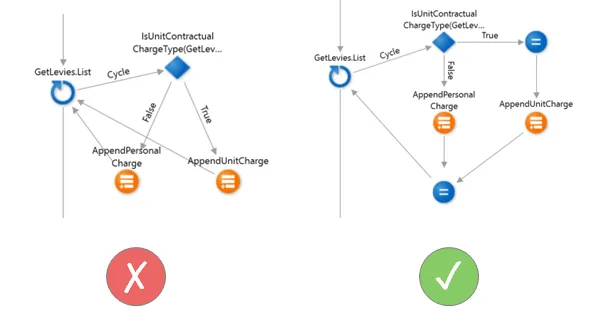
\includegraphics[scale=0.37]{imgs/diretrizes/5.png}
            \caption{Diretriz 5 — Evitar sobreposições}\label{fig:diretriz5}
            \source{\cite{outsystems-style-guide}}
        \end{minipage}%
        \begin{minipage}{.5\textwidth}
            \centering
            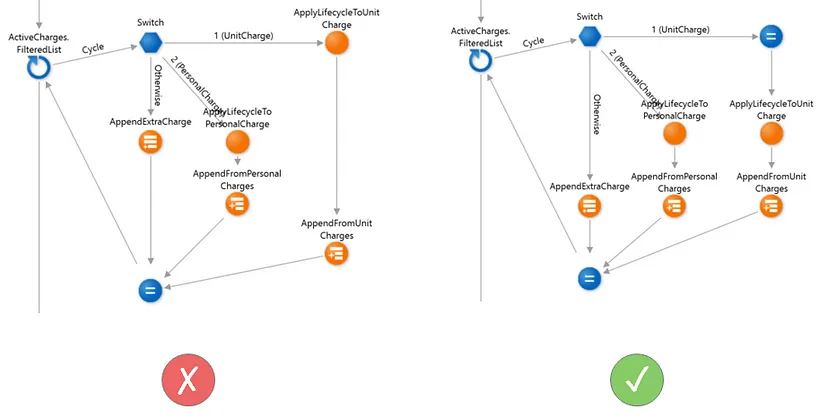
\includegraphics[scale=0.30]{imgs/diretrizes/6.png}
            \caption{Diretriz 6 — Alinhar com intenção}\label{fig:diretriz6}
            \source{\cite{outsystems-style-guide}}
        \end{minipage}
    \end{figure}

    Com estas 6 diretrizes é mais fácil organizar e ler o código da plataforma, e permitirá ter um projeto mais homogéneo e previsível\cite{outsystems-style-guide}.

    % Outlook e ferramentas de desenvolvimento


    % todo, in the Infrestrutura tecnologica na secção que fala de Atlas, referencia também esta secção